% !TeX spellcheck = ru_RU
% !TEX root = vkr.tex

\section{\texorpdfstring{\textsc{Interaction Nets}}{Interaction Nets}}
\label{sec:ins}

Данный раздел является кратким описанием системы \INs{}, более подробно про неё можно узнать в~\cite{lafontInteractionCombinators1997,satoDesignImplementationLowlevel2015, salikhmetovInteractionNetsRussian2013}.

\paragraph{Описание системы.}

\INs{} представляет собой систему переписывания графов.
Зафиксируем множество символов $\Sigma$, которым будем обозначать узлы графа.
Для каждого символа зафиксируем его арность $\ar$, которая будет означать количество \textit{дополнительных} портов символа.
Так, если символ $\alpha \in \Sigma$ имеет арность $\ar(\alpha) = n$, где $n \in \N$, то у символа имеется $n+1$ портов: $n$ дополнительных и один выделенный~--- \textit{главный}.

\begin{center}
    % \begin{tikzpicture}
    %     \inetcell(A){\LARGE $\alpha$}
    %     \inetwirefree(A.left pax)
    %     \inetwirefree(A.right pax)
    %     \inetwirefree(A.pal)
    %     \fill (A.above middle pax) node[anchor=mid] {\dots};
    % \end{tikzpicture}
    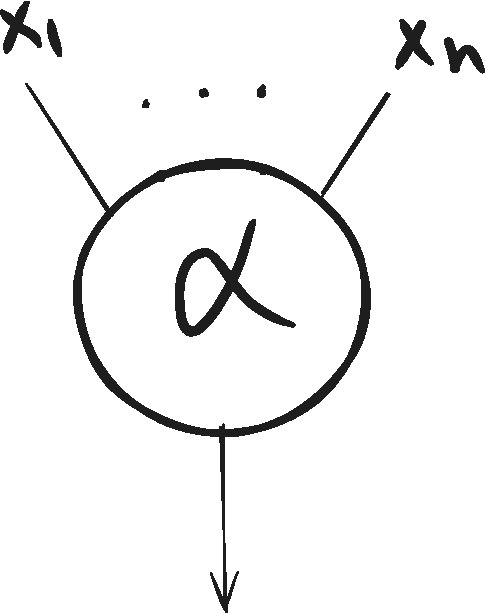
\includegraphics[width=0.125\linewidth]{in_agent.pdf}
\end{center}

Узлы могут изображаться с помощью кругов, треугольников или прямоугольников.
\textit{Сеть}, построенная на $\Sigma$, является неориентированным графом с символами из $\Sigma$ в его вершинах.
Ребра соединяют порты вершин так, что в каждый порт приходит не более одного ребра.
Порт не соединенный ни с одним ребром называется \textit{свободным}, а множество таких портов называется \textit{интерфейсом}.

Пара агентов $(\alpha, \beta) \in \Sigma \times \Sigma$, соединенных своими главными портами называется \textit{активной парой} (редексом).
Правило $((\alpha, \beta) \Longrightarrow N)$ заменяет активную пару $(\alpha, \beta)$ на сеть $N$.
Для каждой пары агентов существует не более одного правила редукции, при этом в процессе редукции интерфейс сохраняется.

\begin{center}
    % \begin{tikzpicture}
    %     \LARGE
    %     \inetcell(A){$\alpha$}[R]
    %     \inetwirefree(A.left pax)
    %     \inetwirefree(A.right pax)
    %     \fill (A.above middle pax) node[anchor=mid] {$\vdots$};
    %     \inetcell[right = of A](B){$\beta$}[L]
    %     \inetwirefree(B.left pax)
    %     \inetwirefree(B.right pax)
    %     \fill (B.above middle pax) node[anchor=mid] {$\vdots$};

    %     \inetwire(A.pal)(B.pal)

    %     \node[right = of B] (arr) {$\Longrightarrow$};

    %     \node[draw, rectangle, right = 1.5 of arr, pin=40:, pin=-40:, pin=140:, pin=-140:, pin={0:$\vdots$}, pin={180:$\vdots$}] (N) {$N$};
    % \end{tikzpicture}
    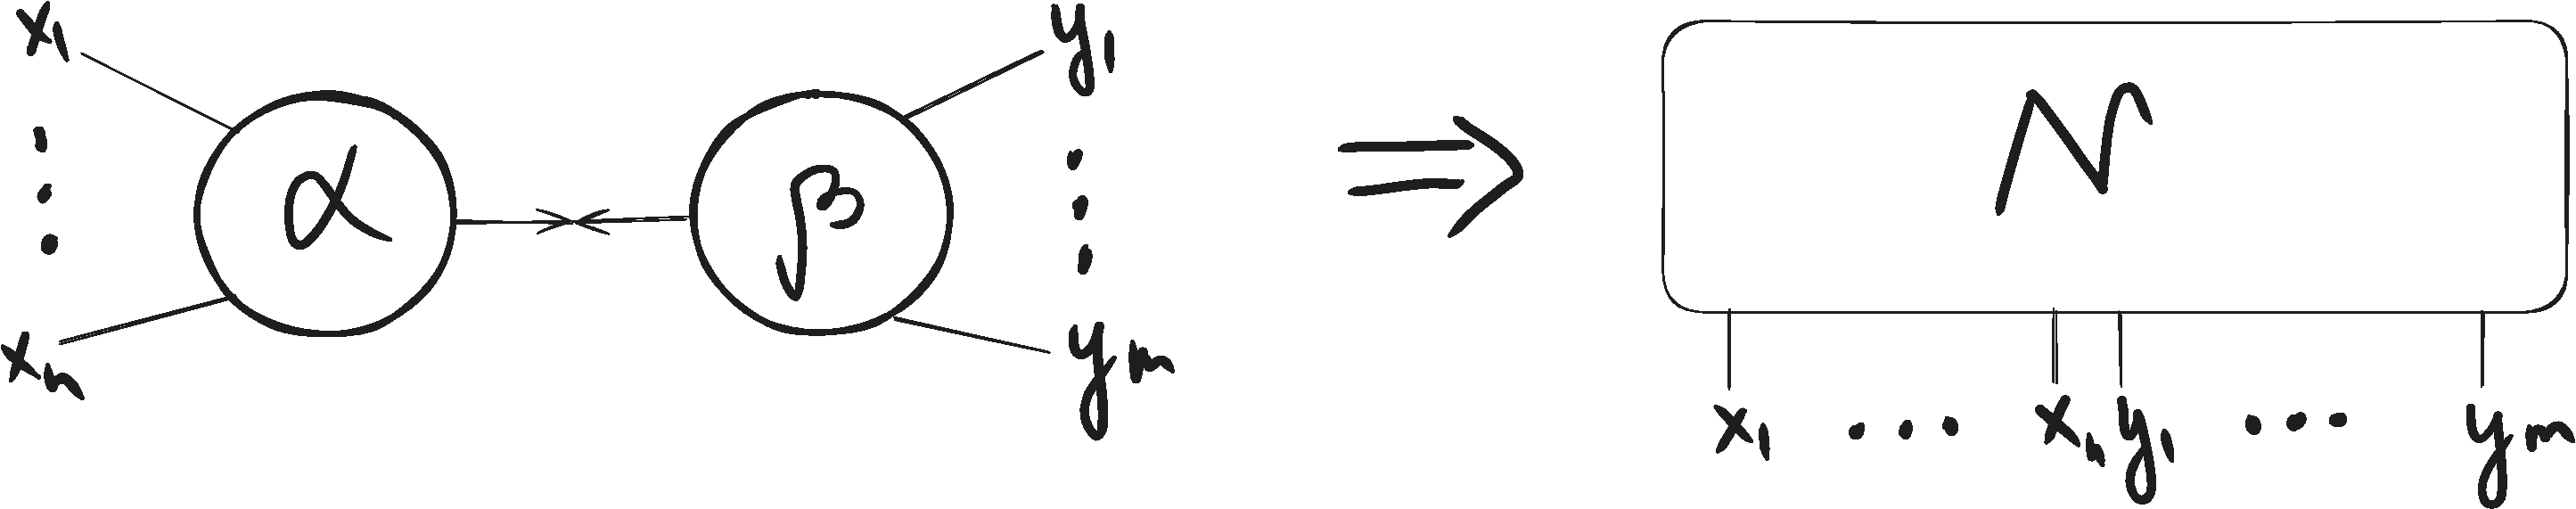
\includegraphics[width=\linewidth]{in_reduction.pdf}
\end{center}

Одним из важных свойств системы является \textit{свойство ромба}: порядок переписываний не важен и все последовательности переписывания имеют одну и ту же длину.
Из этого следуют практически значимые вещи: преобразовывать граф можно в любом порядке, кроме того, это можно делать параллельно.

\paragraph{Выбор базиса агентов.}

Поскольку описание \INs{} не фиксирует набор агентов, пользователю предоставлены большие возможности по созданию собственных наборов и правил их редукции.

Так, например, в статье~\cite{lafontInteractionNets1989} Lafont в качестве примера использует набор агентов $\Sigma = \{\text{Cons}, \text{Nil}, \text{Append}\}$ и правила редукции, соответствующие спискам в функциональных языках программирования.
А в статье~\cite{lafontInteractionCombinators1997} обсуждается базис $\Sigma = \{\gamma, \delta, \varepsilon\}$, который по своим свойствам схож с базисом SKI в $\lambda$-исчислении.

Отдельно можно отметить наличие множества базисов для трансляции $\lambda$-исчисления в \INs{}: \cite{lampingAlgorithmOptimalLambda1990,aspertiBolognaOptimalHigherorder1996,gonthierGeometryOptimalLambda1992,mackieInteractionNetImplementation2011,vincentvanoostromLambdascopeAnotherOptimal2004,sinotCallbyNameCallbyValueTokenPassing2005}.

\paragraph{Стратегия вычислений.}

В отличие от $\lambda$-исчисления, \INs{} не предполагает наличие нескольких стратегий редукции сама по себе.
Тем не менее, поскольку в \INs{} возможно кодировать другие формальные системы, то стратегия редукции может проявится в \INs{} в различных формах записи агентов и правил их редукции.
Так, например, в \INs{} можно закодировать как строгую~\cite{sinotCallbyNameCallbyValueTokenPassing2005}, так и ленивую~\cite{sinotTokenPassingNetsCallbyNeed2006} стратегии для $\lambda$-исчисления.

\paragraph{Типизация.}

\INs{} поддерживает типизацию достаточно интуитивным образом: мы будем помечать порт его \textit{типом} и дополнительно \textit{полярностью}.
Полярность необходима для обозначения, какой порт является \textit{входным}, а какой \textit{выходным}.

Тогда сеть является правильно типизированной, если входы подключены к выходам одного типа.
Правило редукции является правильно типизированным, если
\begin{itemize}
    \item сеть в левой части правила является правильно типизированной;
    \item сеть после редукции остаётся правильно типизированной.
\end{itemize}

Приведём пример из~\cite[раздел~2]{lafontInteractionNets1989}.
Пусть имеется множество типов: \texttt{atom}, \texttt{list}.
Обозначим входные порты, как $\tau^{-}$, а выходные, как $\tau^{+}$.
Тогда набор агентов $\Sigma = \{\text{Cons}, \text{Nil}, \text{Append}\}$ будет типизирован следующим образом:
\begin{center}
    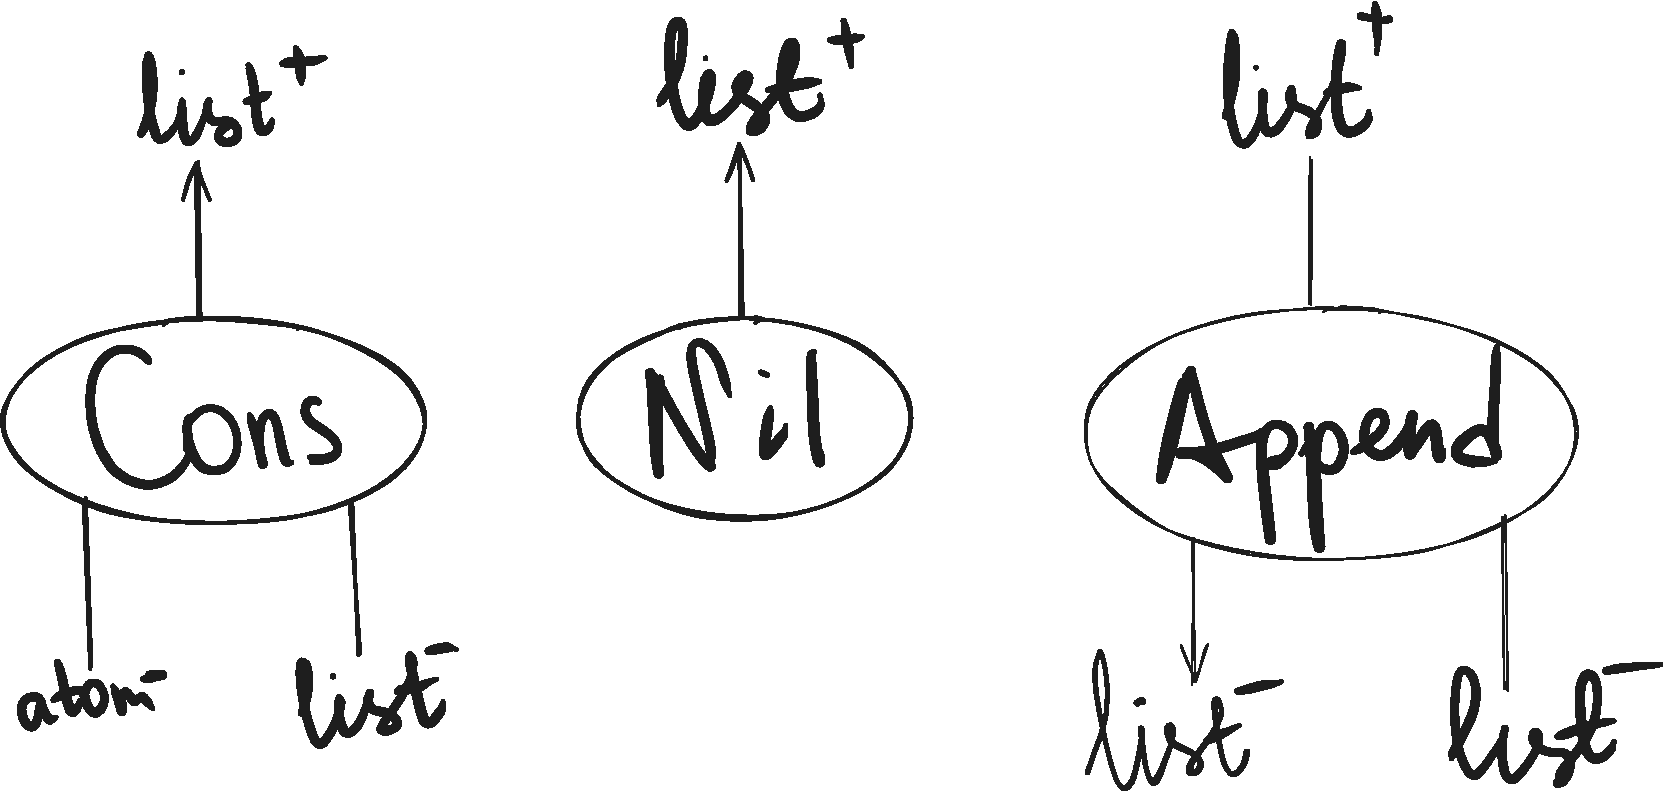
\includegraphics[width=0.6\linewidth]{in_typed.pdf}
\end{center}
А типизированные правила редукции будут выглядеть, как
\begin{center}
    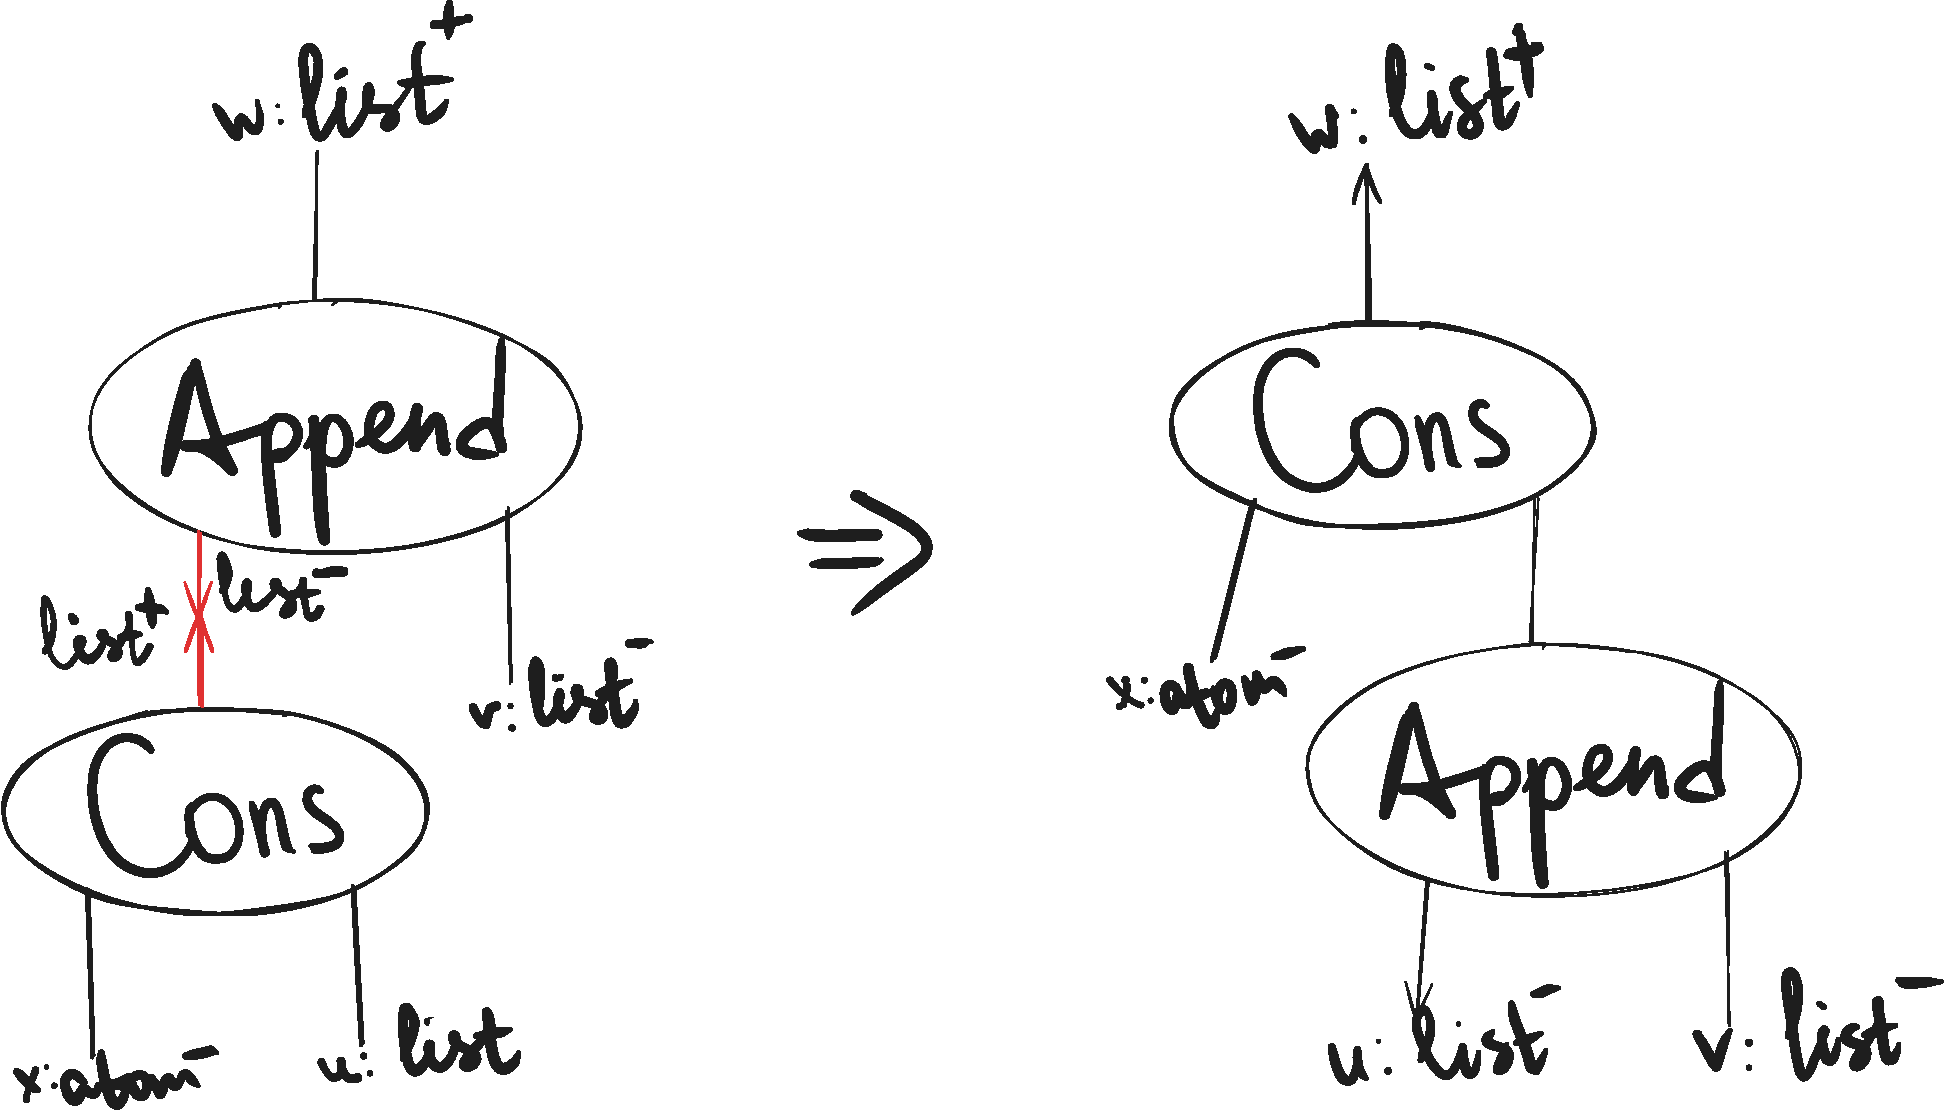
\includegraphics[width=0.6\linewidth]{in_list_red1.pdf}
    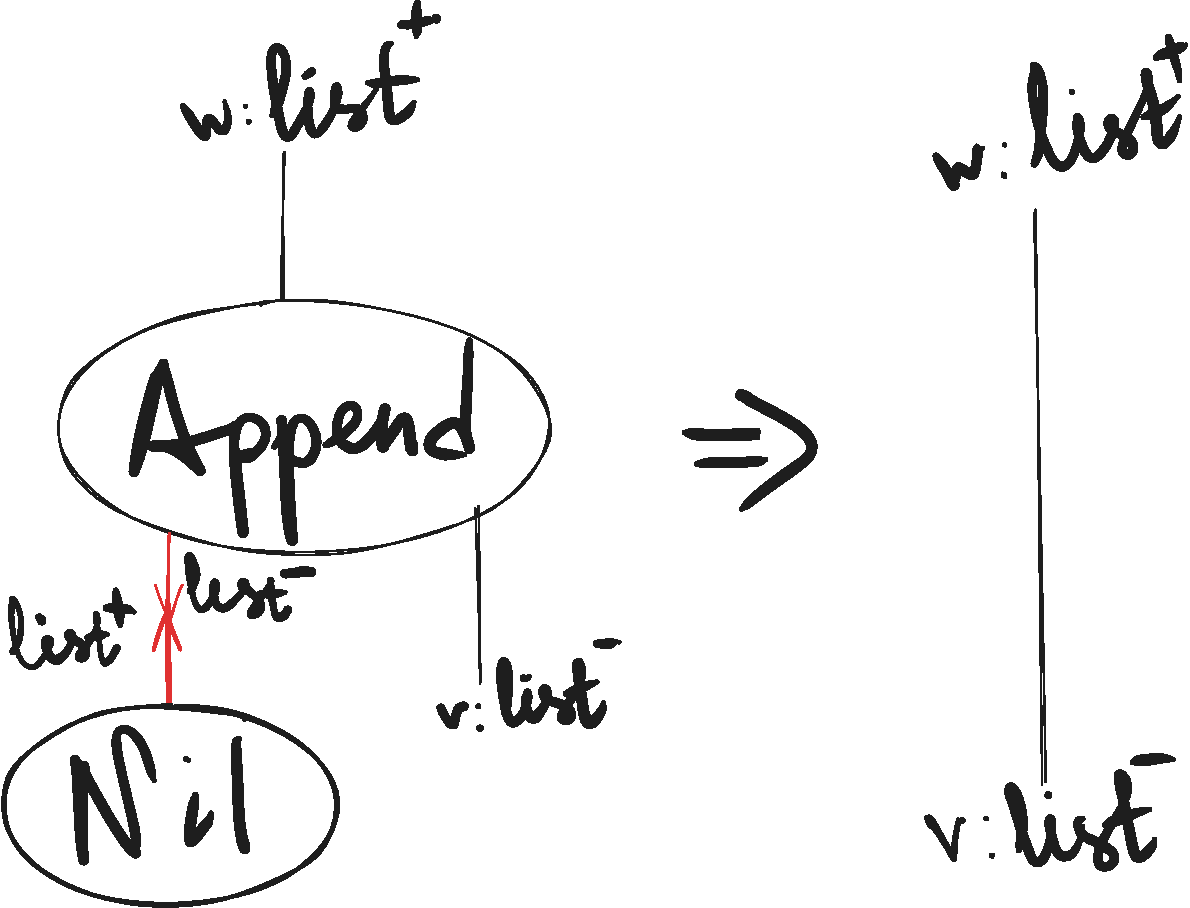
\includegraphics[width=0.4\linewidth]{in_list_red2.pdf}
\end{center}
